\chapter{Evaluation of the RV32I Machine}
\label{Chapter4}

\minitoc

\section{Exploring The Official Tests}
\label{Sec4.1:TESTS}

Since we completed the design of our system its now time to test it so that we can be sure that our work is accurate. To do so, we searched at the official  \href{https://github.com/riscv}{RISC-V GitHub repository} and we found out that they actually provide a toolchain in which, various tests for every architecture can be found. So after installing and configuring their software, we retrieved 37 $.s$ files which were later broke down to .hex and .dump files. So for every instruction in our ISA we have one $.dump$ file and one $.hex$ file. \\

The official RV32I tests have the following structure:
\begin{itemize}
	\setlength\itemsep{-0.1em}
	\item Every test file (for every instruction) has many mini-tests inside it. 
	\item Every mini-test:
		\vspace{-2mm}
		\begin{itemize}
			\setlength\itemsep{-0.1em}
			\item Uses the instruction in which it is dedicated.
			\item On success it updates the $GP$\footnote{Global Pointer} register and moves to the next one.
			\item On failure it jumps to an $ECALL$ instruction which has a specific opcode and terminates the test \footnote{Since the $ECALL$ command is not included to our current ISA, for the purpose of testing we added one extra signal to the $ID$ module which is the $ECALL$ signal. When it comes it simply the signal takes the value 1 and so we understand that the test is finished} .
		\end{itemize}
\end{itemize}

Judging by the way the tests were programmed we conclude that they were designed so that they can guarantee that every possible hazardous scenario for every instruction has been accounted for and avoided. We will mention some cases which we haven't initially considered but we discovered later during testing the pipeline. Alternatively we could try and use our own tests but unfortunately we could not find a stand-alone assembler for our cause. This means that in order to test the system ourselves we would have to program our very own RV32I Assembler...\\
\vspace{-6mm}
\section{Testing Procedure}
\label{Sec4.2:TESTING}
After understanding the testing logic, we used python (version 3) to create a script that takes the $.hex$ file and generates a $.mif$\footnote{Memory Initialization File} which represents the loaded I\$. For $LOADS$ and $STORES$ which had some values stored in D\$ we manually initialized the data cache $.mif$ files for every test. In conclusion we end up with 37 different $.mif$ files for I\$ and also 8 $.mif$ files for D\$ \footnote{There are 5 tests for all the $LOAD$ instructions and 3 for all $STORE$ instructions.}. All that's left now is to run one timing simulation for every test that we have. For our initial tests we used Quartus-II \footnote{Version 9.1sp Web Edition} embedded simulator. Unfortunately the first tests were not successful (as we expected) due to various logic errors in the final structural design and the debug process was not easy because we could not probe the suspicious internal nodes and signals easily using this simulator. We had to modify every file and add extra signals so that they could show up at the simulation. This means alternation to package files and all modules that use the circuit in which we appended a new probing signal to observe. \\

After many debug attempts, we switched to ModelSim where we could easily add and remove every node we wished in the simulation window, something that we made our debug process much easier than it was before. So after various errors we spotted during the testing process we were able to finally find and fix every bug that we found. But for every change we made we couldn't be sure that this change, would not affect previous tests that were completed successfully. So after the final/last changes we made we performed a regression testing, meaning that we run all the tests again. The results were satisfying, since every test was completed successfully. 
\vspace{-4mm}
\subsection{A Test Example}
\label{SubSec4.2.1:EXAMPLE}

We will now showcase a sample of our testing process. This test concerns the "ADDI" command. All we need is just the $.dump$ file so that we can understand and follow the simulation and also we need the simulation window. The "ADDI" test file has 25 mini-tests so we cannot go through all of them. We will present the first of those tests and its prosperous results. 

\begin{figure}[h!]
	\begin{center}
		\fbox{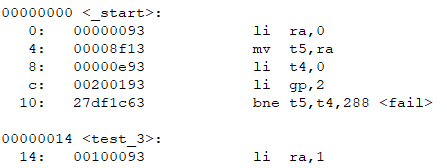
\includegraphics[width=0.7\textwidth]{ADDITEST2}}
		\caption{ADDI test \#2.}
		\label{Image4.1}
	\end{center}
\end{figure}

\clearpage

\begin{figure}[h!]
	\begin{center}
		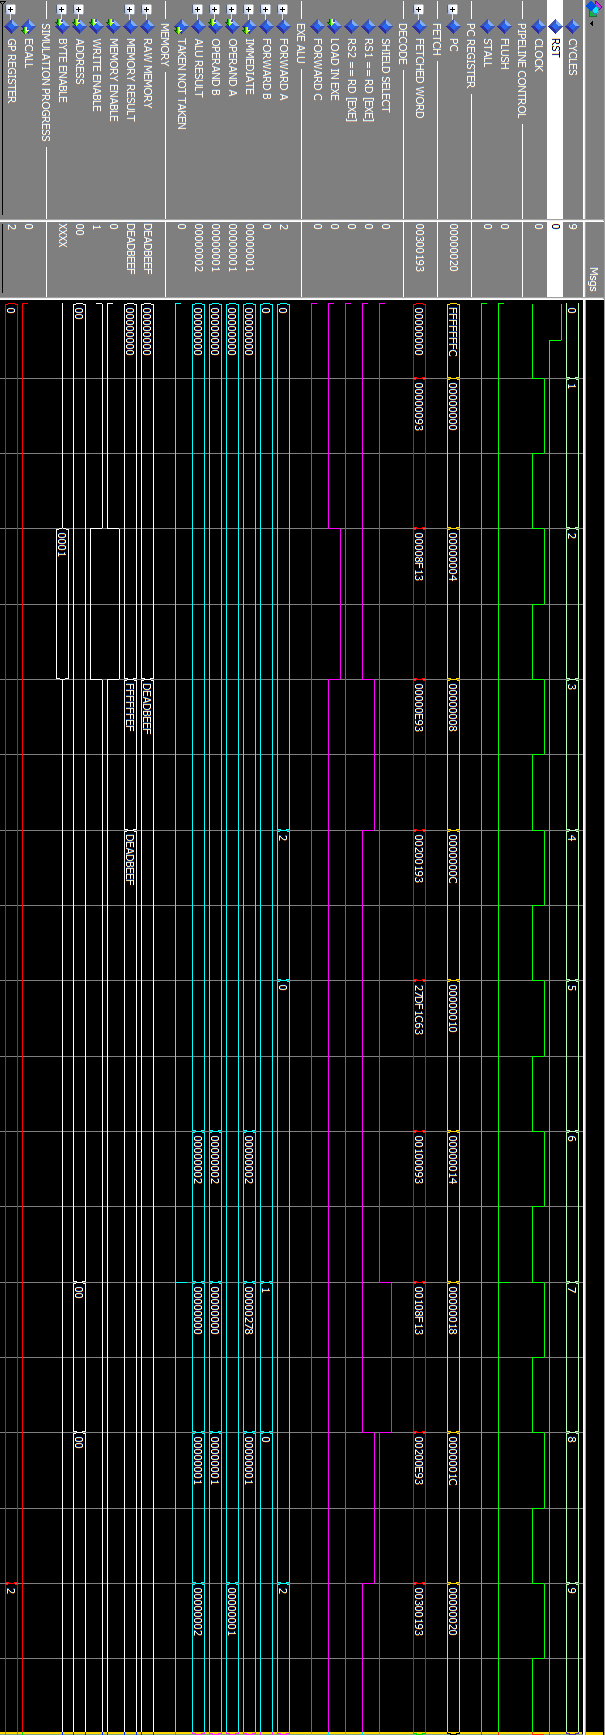
\includegraphics[height = 0.9\textheight,width=1\textwidth]{MODELSIM}
		\caption{ModelSim simulation of the "ADDI" test \#2.}
		\label{Image4.2}
	\end{center}
\end{figure}

\clearpage
\subsubsection{About the Figure \ref{Image4.1}}
The Load Immediate ($li$) command is a pseudo-operation which translates to: $addi$ $rd$, $x0$ $immediate$ register. The Move $mv$ command is also a pseudo-operation which translates to $addi$ $rd$, $rs1$, $0$. So all this test does, is to load to register \$ra the immediate 0, then copy its value to register \$t5. Furthermore, it loads to register \$t4 the zero immediate again and to register \$gp \footnote{Global Pointer, this register gets updated with the test's id number. So if the register is written with all the mini-test ids we can tell that all the tests were successful} it loads the id number of the test (immediate 2). Finally it conducts a branch which ends to the fail section if it is Taken, and the branch simply compares the value of \$t5 and \$t4 registers which should have the same value if everything went according to plan. If the test succeeds then the next command that we should see being fetched it would be the $00100093$ $li$. 

\subsubsection{About the Figure \ref{Image4.2}}

We will pair the simulation waves shown in the Figure with a Pipeline diagram to make it easier and more lucid.\\
\vspace{4mm}
\begin{threeparttable}
	\footnotesize
	\begin{tabular}{|l|c|c|c|c|c|} \hline
		\setrow{\bfseries} Clock Cycle& \setrow{\bfseries} $IF$ & \setrow{\bfseries} $ID$ & \setrow{\bfseries} $EXE$ & \setrow{\bfseries} $MEM$ & $WB$ \\\hline
		0 & li ra, 0  & - & - & - & - 	   \\\hline
		1 & mv t5, ra & li ra, 0  & - & - & - \\\hline
		2 & li t4, 0  & mv t5, ra & li ra, 0 & - & - \\\hline
		3 & li gp, 2  & li t4, 0  & mv t5, ra & li ra, 0  & - \\\hline
		4 & bne t5, t4, 288 & li gp, 2 & li t4, 0 & mv t5, ra & \cellcolor{brightgreen} li ra, 0 \\\hline
		5 & li ra, 1  & bne t5, t4, 288 & li gp, 2  & li t4, 0   & \cellcolor{brightgreen} mv t5, ra \\\hline
		6 & - & li ra, 1  & \cellcolor{brightgreen}bne t5, t4, 288 & li gp, 2  & \cellcolor{brightgreen} li t4, 0  \\\hline
		7 & - & - & li ra, 1  & - & \cellcolor{brightgreen} li gp, 2 \\\hline
		8 & - & - & - & li ra, 1  & - \\\hline
			
	\end{tabular}
	
	\begin{tablenotes}
	\footnotesize
	\item Notes:
	
	\underline{\textbf{\textcolor{brightgreen}{$\rightarrow$}}} The command is completed at the next clock cycle.
	\captionof{table}{Pipeline Diagram of test \#2}
	\label{Table4.1}
	\vspace{5mm}
	\end{tablenotes}

\end{threeparttable}

The legend of the Figure \ref{Image4.2} monitors some signals that we have selected for display. Note that at the bottom row, there is a signal dedicated to the \$gp register that gets updated with the value 2 at clock cycle 9 as we expected to happen. But it would get updated even if the branch was taken and the test failed. What makes sure that the test is successful is that when the branch reaches its final stage (the $EXE$ stage) does not generate a $TAKEN$ and therefore there is no $FLUSH$ signal to empty the previous pipeline registers. 

\clearpage

\section{Problems Indicated by Testing}
\label{SubSec4.3:PROBS}




 